\subsubsection*{LWE problem}
There are multiple equivalent definitions of this problem. We adopt the notation and approach introduced in the original paper by Regev. In this section, we will mainly focus on the parts that are the most relevant for our study of ring-LWE such as \ref{classical} and \ref{s-to-d}. 

The problem is parametrized by positive integers $n$, $m$\footnote{As will be seen later, $m$ plays virtually no role in the problem definition and is usually omitted.} and prime $q$, as well as a discrete error distibution $\chi$ over $\Z_q$. It is now defined as follows. We are given $m$ equations of the form $(\bm{a}_i, b_i = \langle \bm{a}_i, \bm{s} \rangle + e_i)$ and are asked to find the vector $\bm{s} \in \Z_q^n$. Here, $\bm{a}_i$ are chosen uniformly and independently from $\Z_q^n$, $b_i \in \Z_q$ and $\langle \cdot, \cdot \rangle$ denotes the usual dot product. The errors $e_i$ are obtained by sampling independently from the probability distribution $\chi : \Z_q \rightarrow \R_{> 0}$ on $\Z_q$. We will denote the problem of recovering $\bm{s}$ from such equations, by $\text{LWE}_{q, \chi}$ (learning with errors).

\begin{example}\label{lwe_ex}
        Given as input this set of equations, LWE asks us to recover the vector $\bm{s} = (s_1, s_2, s_3, s_4) \in \Z_{17}^4$. In this case $n = 4$, $q=17$ and the error distribution is giving us $e_i < 1$ for each $i \in [m]$. 
\begin{align*}
        0s_1 + 11s_2 +8s_3 + 2s_4 & \approx_{e_1} 3 \, \mod 17\\
        9s_1 +  3s_2 + 7s_3 + 0s_4 & \approx_{e_2} 16 \, \mod 17\\
        1s_1 +  15s_2 + 9s_3 + 5s_4 & \approx_{e_3} 16 \, \mod 17\\
        0s_1 +  0s_2 + 13s_3 + 5s_4 & \approx_{e_4} 1 \, \mod 17\\
\end{align*}
In this case, $\bm{s} = (7, 13, 12, 16)$. Note that if not for the error, the secret would be very easy to find. Given about $n$ equations, we could recover $\bm{s}$ in an efficient way using Gaussian elimination. Inducing the error is what seems to render the problem untraceable for modern day algorithms.
\end{example}
The central part of \cite{regev} revolves around proving the hardness of LWE. Specifically, that for appropriately chosen $q$ and $\chi$, a \textit{quantum}\footnote{In fact, quantum reduction is used only in the small part of the whole proof.} reduction algorithm exists that approximates worst-case lattice problems. The following is the main result presented in the paper. 

\begin{theorem}[\cite{regev}, Theorem 1.1]\label{main}
        Let $n$, $q$ be positive integers and $\alpha \in (0, 1)$ be such that $\alpha q > 2 \sqrt{n}$. If there exists an efficient algorithm that solves $\text{LWE}_{q, \Psi_{\alpha}}$, then there exists an efficient quantum algorithm that approximates the decision version of the shortest vector problem (\prob{GapSVP}$_{\gamma}$) and the shortest independent vectors problem (\prob{SIVP}$_{\gamma}$) to within $\gamma = \tilde{O}(n/\alpha)$ in the worst case on any lattice of dimension $n$. 
\end{theorem}

Let us unwrap this statement. As said before, we need an appropriate choice of paramenters to obtain our results and $\alpha > 2\sqrt{n}/q$ is one of those choices (and requirements). It specifies the shape of the $\Psi_{\alpha}$ distribution. This one is almost identical to the discrete Gaussian distribution over $\Z_q$ that is centered around 0 with standard deviation $\alpha q$. It will be used to sample the errors with some nice and predictable properties. Later, by the end of this section, we will also show that in fact, there is sort of an equivalence between drawing them from continuous and discrete distributions.

The theorem can be rephrased as follows. Imagine that we have an efficient algorithm that solves the $\text{LWE}_{q, \Psi_{\alpha}}$. Then, there exists a quantum solution to worst-case lattice problems, namely \prob{GapSVP} and \prob{SIVP}. Since we strongly believe that \prob{GapSVP} and \prob{SIVP} are difficult to solve (\cite{svp-hard}, \cite{reductions}, \cite{cvp-hard}, \cite{lbc}) we are left with a difficult, yet efficient way to share secrets. Oded Regev proceeds to prove this using various lemmas and results from few areas of mathematics like probability, lattice theory and quantum computing. We will now present selected proofs and outline of the whole the approach.

\subsubsection{Preliminaries}
Here we will define essential and convenient definitions and lemmas concerning Gaussian distributions lattices and lattice-related problems. Note that no algebraic number theory is needed for this section as we work exclusively over $\R^n$ and $\Z^n_q$ for $q$ an integer (it is only required for $q$ to be prime in Theorem \ref{s-to-d}, otherwise no assumptions are made). 

\paragraph{Gaussians}
The ideas presented here heavily rely on the distribution of errors. The most important distribution we will be using is the \textit{Gaussian distribution} (also called the normal distribution). For some vector $\bm{x}$ and $r>0$, we define the Gaussian function as
\[ \rho_r (\bm{x}) := \text{exp}(- \pi ||\bm{x}/r||^2) \]
where exp($y$) stands for $e^y$. We will also denote $\rho_1$ by $\rho$. By normalizing it, we obtain the $n$-dimensional Gaussian distribution
\[\D_r = \rho_r \Big/ \Big( \int_{\bm{s} \in \R^n} \rho_r(\bm{s}) d\bm{s} \Big) = \rho_r \cdot r^{-n}. \]
We can also define the \textit{discrete Gaussian distribution} $\D_{\Ll, r}$ over a lattice $\Ll$ (or any countable set $A$ for that matter) by
\begin{equation} \D_{\Ll, r}(\bm{x}) = \frac{\rho_r(\bm{x})}{\rho_r(\Ll)} \end{equation}
where $\rho_{A, r}(\bm{x}) = \sum_{\bm{x} \in A} \rho_r(\bm{x})$ is an extension of $\rho_r$ to a countable set.

\krzys{i dont think ill include this part about Psi beta at all}
In order to avoid making our proofs depend on the specific choice of modulus $q$, we now define the family of Gaussian distributions over $\T = \R/\Z = [0,1)$ - a periodization of the normal distribution. More specifically, following \cite{regev}, for $\beta \in \R_{> 0}$ define $\Psi_{\beta}$ as the distribution on $\T$ obtained by sampling from a normal variable with mean 0 and standard deviation $\frac{\beta}{\sqrt{2\pi}}$ and reducing the result modulo 1,
\begin{equation} \forall r \in [0,1), \Psi_{\beta}(r) := \sum_{k = -\infty}^{\infty} \frac{1}{\beta} \cdot \text{exp} \bigg(- \pi \Big(\frac{r-k}{\beta}\Big)^2\bigg). \end{equation}
\krzys{also, it turns out, that for whatever value of $r$ we pick, the result of that sum is always $|\beta|/\beta = 1$?????}
We will, for the sake of clearer notation, be a bit vague about the doman of $\Psi_{\beta}$. This is because sampling from $\Psi_{\beta}$ with parameter $\beta$, that is defined over $\T = [0,1)$ is equivalent to sampling from $\Psi_{q \beta}$ over $\Z_q$. \krzys{i am very hesitant about this statement - need to check if thats true}

We also need to define \textit{distretization} of a probability density function for our cryptosystem introduced later. For an arbitrary probability density function $\phi~:~\T~\to~\R_{>0}$ and an integer $q \geq 2$, we define its discretization $\bar{\phi} : \Z_q \rightarrow R_{>0}$ as the discrete probability distribution obtained by sampling from $\Psi$, multiplying by $q$, and rounding to the closest integer modulo $q$. More formally,
\begin{equation} \bar{\phi}(i) = \int_{(i -1/2)/q}^{(i + 1/2)/q} \phi(x) dx \end{equation}

Lastly, following the definition given in \cite{lbc}, we define the \textit{statistical distance} as follows.
\begin{definition}[Statistical distance]
        Let $X,Y$ be two random variables over a countable set A. The statistical distance between them is defined as
        \[\Delta(X,Y) = \sum_{a \in A} \Big| \Pr\{X = a\} - \Pr\{Y = a\} \Big|.\]
Similarly, if $\varphi_X, \varphi_Y$ are the \textit{probability density} functions over $\R^n$ of $X$ and $Y$ respectively, then
\[ \Delta(\varphi_X, \varphi_Y) = \int_{\bm{s} \in \R^n} \Big| \varphi_X(\bm{s}) - \varphi_Y(\bm{s}) \Big|d\bm{s}. \]
\end{definition}
It can be interpreted as a measure of how much apart two distributions are from each other. It is indeed not hard to show that this definition satisfies the properties of a distance function. We will be using this tool to measure how our elements are behaving, for example, in Lemma \ref{s-to-d}.

\paragraph{Smoothing parameter}
One of the most important concepts invoked in the paper is the so called \textit{smoothing parameter} $\eta$ of a lattice $\Ll$. It was first introduced in \cite{smoothing} and has proven useful over the course of the years. The definition is quite technical as it makes use of the dual rather than the lattice itself. The intuition behind it could be obtained by imagining the following. Pick an element from your favourite lattice $\Ll$. If one now picks a ``noise'' vector from a Gaussian distribution with width at least as large as the smoothing parameter, the resulting distribution is very close to uniform. The precise definition is as follows.
\begin{definition}[Smoothing parameter]\label{smoothing}
        For an $n$-dimensional lattice $\Ll$ and positive real $\epsilon > 0$, we define the smoothing parameter $\eta_{\epsilon}(\Ll)$ to be the smallest $s$ such that $\rho_{1/s}(\Lld \backslash \{\bm{0}\}) \leq \epsilon$.
\end{definition}
In other words, $\eta_{\epsilon}(\Ll)$ is the smallest $s$ such that a Gaussian measure scaled by $1/s$ on the dual lattice $\Lld$ gives all but $\epsilon/(1+\epsilon)$ of its weight to the origin - \cite{regev}. Note that we need to use the dual in the definition because we cannot really make sense of the ``longest'' element of the lattice $\Ll$ as there is none. Instead, we look at the shortest element of the dual $\Lld$ which we know exists. $\epsilon$ is our desired tolerance and as the name suggests, it is usually taken to be very small (in our cases, a negligible function of $n$). It is also worth noting that $\eta_{\epsilon}(\Ll)$ is a continuous function of $\epsilon$. 

In the Figure \ref{smoothing-1}, there are plotted four Gaussians. The first one has very small deviation and assigns most of its values to the origin. The second one, with the deviation $\sqrt{10}$ times the size of the first one, looks a bit more \textit{smooth} and continuous. Finally, the last distribution is almost uniform or ``flat''. For an appropriate choice of $\epsilon$, the smoothing parameter will lay somewhere between those four values of $r$.

\begin{figure}[ht]
        \centering
                \begin{subfigure}{.5\linewidth} 
                \centering
                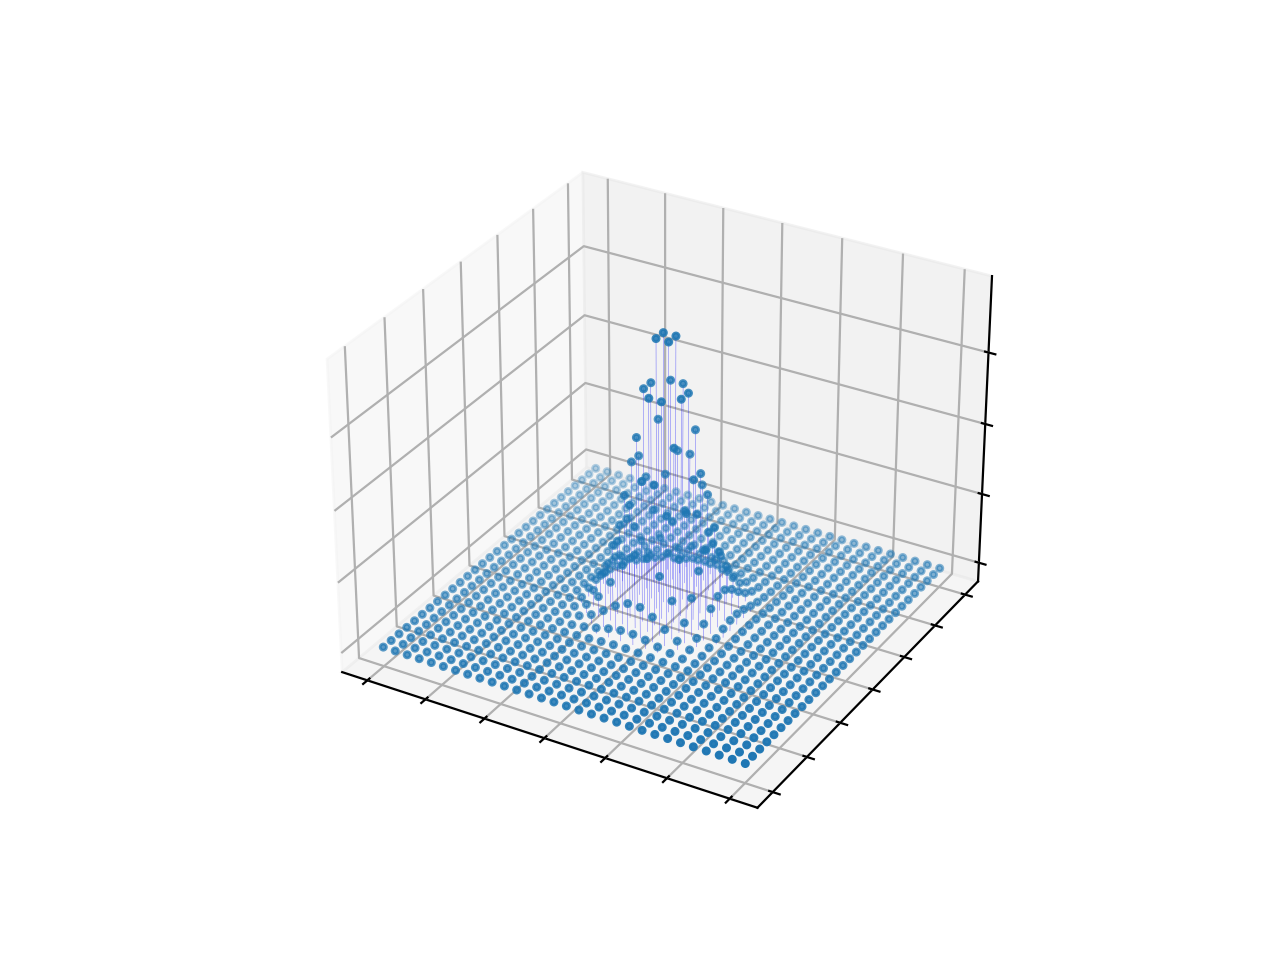
\includegraphics[scale=0.5]{gaussian-1.png}
                \caption{$r = 0.2$}
        \end{subfigure}%
        \begin{subfigure}{.5\linewidth}
                \centering
                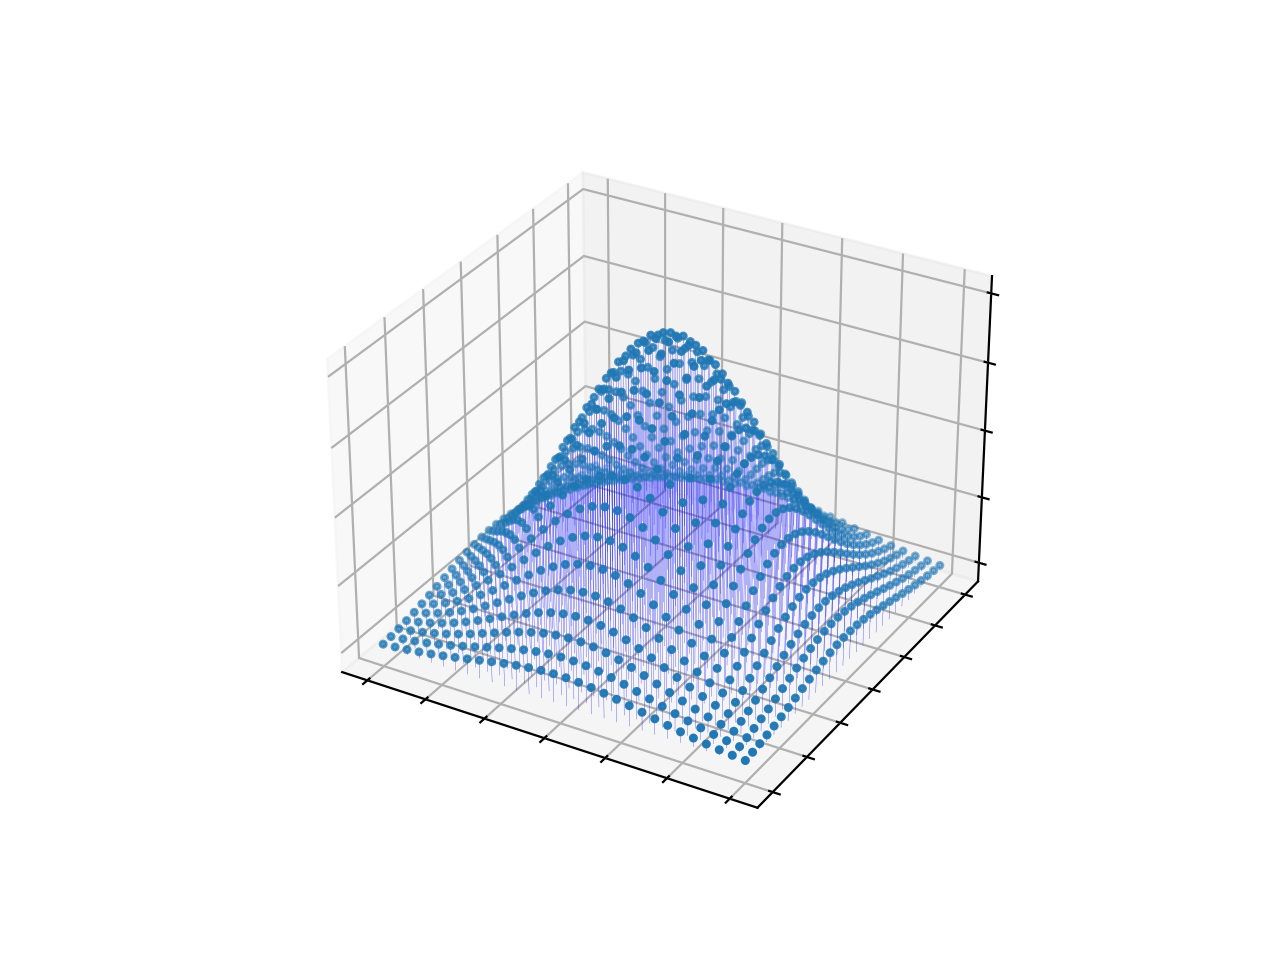
\includegraphics[scale=0.5]{gaussian-2.png}
                \caption{$r = 2$}
        \end{subfigure}
\end{figure}

\begin{figure}[h]
        \centering
                \begin{subfigure}{.5\linewidth} 
                \centering
                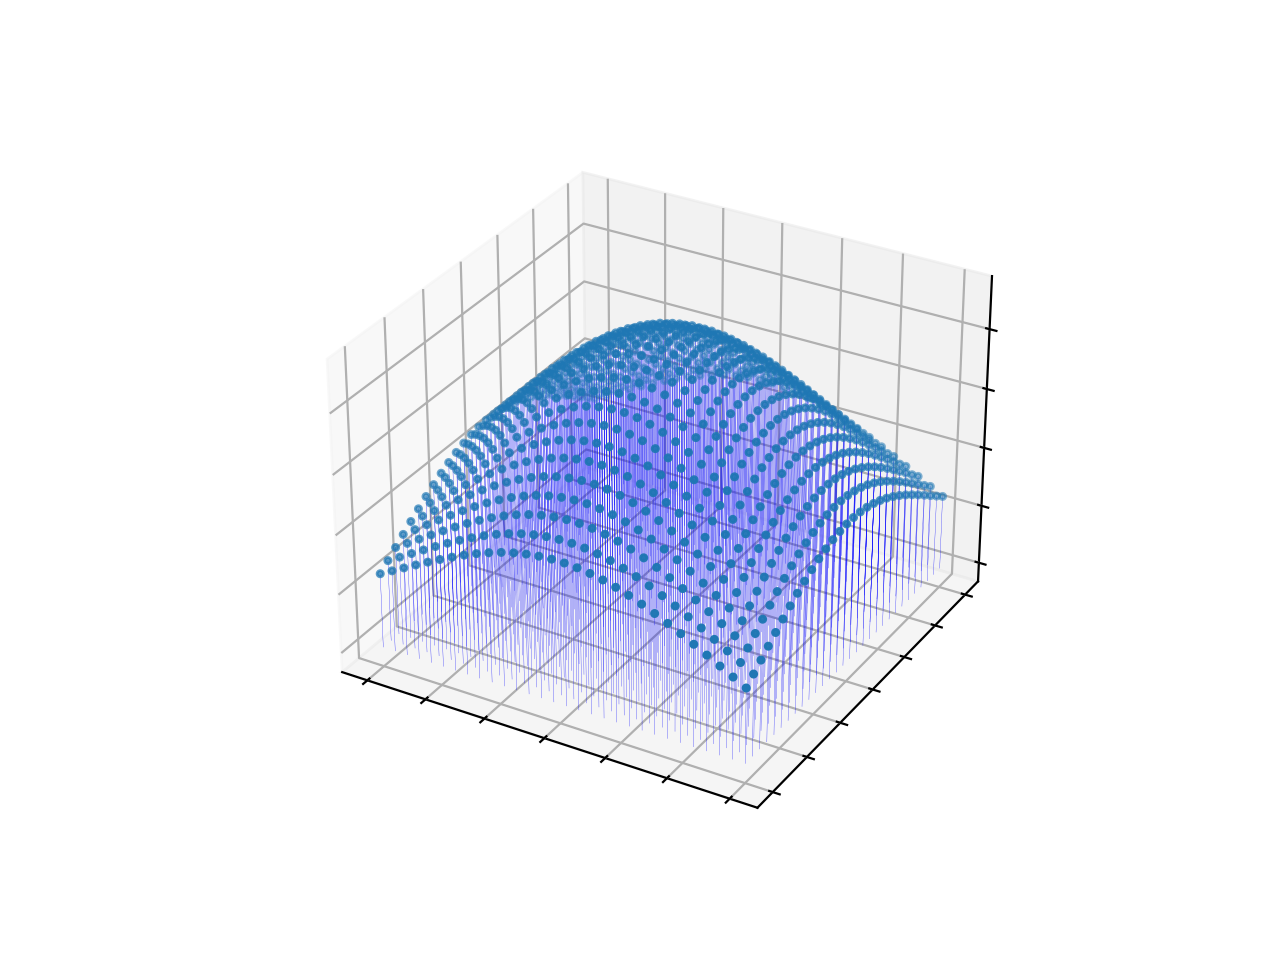
\includegraphics[scale=0.5]{gaussian-3.png}
                \caption{$r = 7$}
        \end{subfigure}%
        \begin{subfigure}{.5\linewidth}
                \centering
                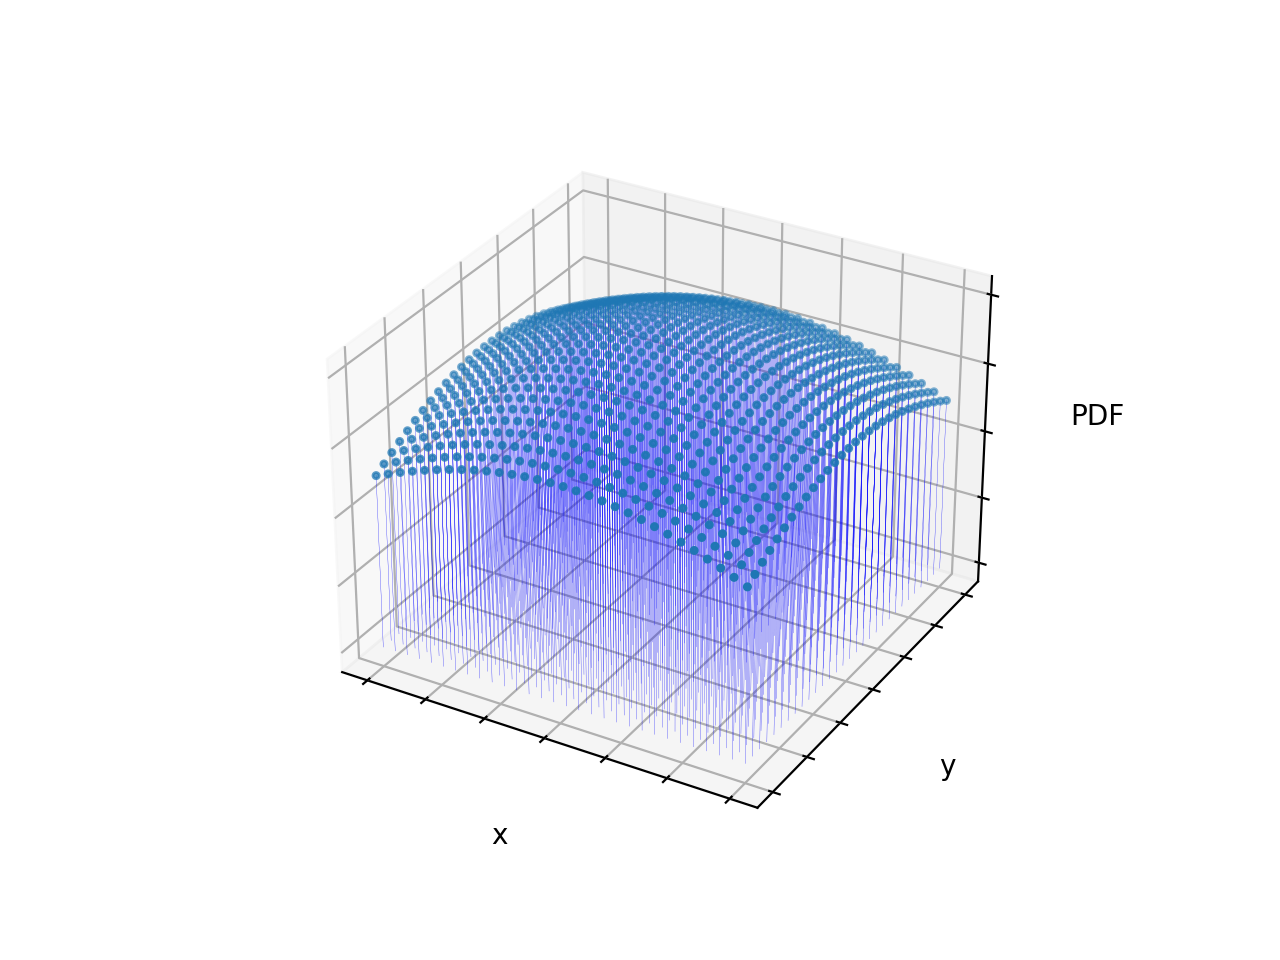
\includegraphics[scale=0.5]{gaussian-4.png}
                \caption{$r = 20$}
        \end{subfigure}
        \caption{2-dimensional Gaussian with standard deviation $r$. The $z$-axis represents the probability.}
        \label{smoothing-1}
\end{figure}
\begin{proposition}[Sum of Gaussians]\label{gauss_sum}
If $X_1, X_2, \cdots, X_n$ are mutually independent normal random variables with means $\mu_1, \mu_2, \cdots, \mu_n$ and variances $\sigma_1, \sigma_2, \cdots, \sigma_n$, then the linear combination
\[ Y = \sum_{i \in [n]} c_i X_i \]
follows the normal distribution
\[ \mathcal{N}\biggl(\sum_{i \in [n]} c_i \mu_i, \sum_{i \in [n]} c^2_i \sigma^2_i\biggr). \]
\end{proposition}
\paragraph{Problems}
We will now define problems related specifically to the LWE. First, let us define the distribution induced by LWE. 
\begin{definition}[LWE distribution]\label{lwe-distr}
        Let $q \geq 2$ be some integer, and let $\chi : \Z_q \rightarrow \R_{>0}$ be some probability distribution on $\Z_q$. Let $n$ be an integer and let $\bm{s} \in \Z_n^q$ be a vector. We define $A_{\bm{s},\chi}$ as the distribution on $\Z_n^q \cross \Z_q$ obtained by choosing a vector $\bm{a} \in \Z_q^n$ uniformly at random, choosing $e \in \Z_q$ according to $\chi$, and outputting $(\bm{a}, \langle \bm{a}, \bm{s} \rangle + e)$, where additions are performed in $\Z_q$, i.e., modulo $q$. In parallel, we define $U$ as the uniform distribution on $\Z_q^n \cross \Z_q$.
\end{definition}

There are two types of problems we can define over LWE - the \textit{search} and \textit{decision}. We will prove at the end of this section that they are in fact equivalent, i.e. there exists a reduction between them. Search-LWE is asking us to find $\bm{s}$ from a list of samples distributed according to $A_{\bm{s}, \chi}$ for some unknown $\chi$. Similarly, the \textit{decision} asks us to distinguish samples $(\bm{a}, b)$ that were draw from either $A_{\bm{s}, \chi}$ or the uniform distribution. Although not present in the original paper, we define them formally here.
\begin{definition}[Search-LWE]\label{slwe}
        Given access to arbitrarily many samples from the $A_{\bm{s}, \chi}$, find $\bm{s}$.
\end{definition}
\begin{definition}[Decision-LWE]\label{dlwe}
        Given access to arbitrarily many samples from the $A_{\bm{s}, \chi}$ and the same amount of samples from the uniform distribution, distinguish (with non-negligible advantage) between them.
\end{definition}
The following is used as an intermediate step in our reduction to \prob{SIVP}. The acronym \prob{DGS} stands for \textit{discrete Gaussian sampling} problem and is concerned exactly with that - to find a sample from the normal distribution over our lattice. Formally:
\begin{definition}[\prob{DGS}]\label{dgs}
        Given an $n$-dimensional lattice $\Ll$ and a number $r \geq \sqrt{2}n \cdot \eta_{\epsilon}(\Ll)/\alpha$, output a sample from $\D_{\Ll,r}$
\end{definition}

\subsubsection{Hardness of search LWE}
In this section we will base the hardness of LWE on some hard lattice problems like \prob{SIVP} following the approach in \cite{regev}. We will put an emphasis on the parts that require the most adjustment when trying to prove the same results for ring-LWE in the next section.

Recall what we want to prove, that being able to solve $\text{LWE}_{q, \chi}$ implies that we are able to solve standard worst-case lattice problems like \prob{SIVP}. To achieve this, we need to proceed in steps, in other words, we perform reductions from one problem to another. From this point on, a probabilistic algorithm which solves a given $\text{LWE}_{q, \chi}$ instance, will be called an LWE-\textit{oracle} (or, when there is no confusion, simply an oracle).

The high-level version of the proof is as follows. Let us assume that we have such an oracle that solves $\text{LWE}_{q, \chi}$ on a lattice $\Ll$ just like in the assumption. The procedure is based on the so called \textit{iterative step} (IS). It is repeatedly used to reduce our LWE problem to the problem of sampling from the  discrete Gaussian distribution on $\Ll$. As it turns out, it is indeed sufficient to solve the \prob{DGS} problem (Definition \ref{dgs}). Intuitively, if we have enough samples from the Gaussian distribution of some small radius $r$ around our lattice, we can use it to obtain short lattice vectors. Indeed, if we call the \prob{DGS} oracle enough times we can prove, that with very high probability, there are $n$ linearly independent vectors among the samples returned by oracle - thus, a solution to \prob{SIVP}.

On each of the iterations, the IS is using the oracle to produce discrete Gaussian samples of smaller and smaller radius around our desired \textit{closest vector}. Once we have a sample with radius small enough, we can use that to solve \prob{DGS} and use one more step which is the reduction from \prob{DGS} to the \prob{GapSVP} and \prob{SIVP} as required in Theorem \ref{main}.

\begin{center}
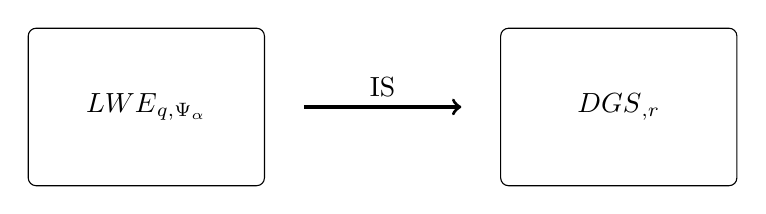
\begin{tikzpicture}
% Define the left box
\draw[rounded corners=1mm] (0,0) rectangle (3,2);
\node at (1.5,1) {$\text{LWE}_{q, \Psi_{\alpha}}$};

% Define the right box
\draw[rounded corners=1mm] (6,0) rectangle (9,2);
\node at (7.5,1) {$\text{DGS}_{\Ll, r}$};

% Define the arrow between the boxes
\draw[->, very thick] (3.5,1) -- node[above] {IS} (5.5,1);
\end{tikzpicture}
\end{center}

The algorithm can be divided into two basic steps, the \textit{classical} step and the \textit{quantum} step. First, given some polynomial number $n^c$ (where $c$ is some positive integer) of samples from a discrete Gaussian on $\Ll$ with some (large enough) parameter $r$, we us the first step to obtain a solution to a \prob{CVP} on the dual lattice $\Lld$ to within some (smaller than the initial $r$) distance. We then use this solution along with the second step - the quantum algorithm - to obtain $n^c$ samples from a dicrete Gaussian with parameter $r' < r$. Iterating these steps polynomial amount of times, we finally get $n^c$ samples from D$_{\Ll, r''}$ where $r'' \ll r$. We simply pick one of those samples to solve the \prob{DGS}$_{\Ll, r}$ and we are done.

The full picture now stands as follows. We begin with a assumed solution to LWE and we end up with a solution to some (conjured) hard lattice problems like \prob{SIVP} to within some tolerance $\gamma = \tilde{O}(n/\alpha)$.

\begin{center}
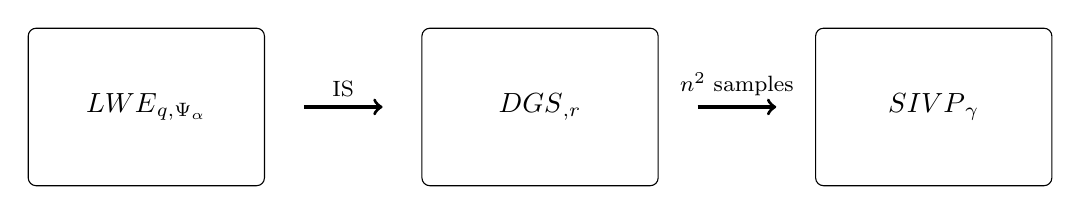
\begin{tikzpicture}
\draw[rounded corners=1mm] (0,0) rectangle (3,2);
\node at (1.5,1) {$\text{LWE}_{q, \Psi_{\alpha}}$};

\draw[->, very thick] (3.5,1) -- node[above] {\footnotesize IS} (4.5,1);

\draw[rounded corners=1mm] (5,0) rectangle (8,2);
\node at (6.5,1) {$\text{DGS}_{\Ll, r}$};

\draw[->, very thick] (8.5,1) -- node[above] {\footnotesize $n^2$ samples} (9.5,1);

\draw[rounded corners=1mm] (10,0) rectangle (13,2);
\node at (11.5, 1) {$\text{SIVP}_{\gamma}$};

\end{tikzpicture}
\end{center}
We will now focus on the first step of the reduction from LWE to \prob{DGS} as it is what is altered the most in the ring-LWE hardness proof. This, however, will follow in the next section.

The following statement (Theorem 3.1 in \cite{regev}) is the core of the hardness results of (search) LWE. Given an oracle for LWE, there exists an algorithm that gives us samples from discrete Gaussian distribution which in turn can yield us a solution to the \prob{CVP}. For example, later we will show the equivalence between search-LWE and decision-LWE (Theorem \ref{s-to-d}). This is an important result as it is usually much easier to construct cryptographic schemes based on some \textit{decision} version of a problem rather than the \textit{search}.

\begin{theorem}\label{heart}
        Let $\epsilon = \epsilon(n)$ be some negligible function of $n$. Also, let $q = q(n)$ be some integer and $\alpha = \alpha(n) \in (0, 1)$ be such that $\alpha q > 2\sqrt{n}$. Assume that we have access to an oracle W that solves $\text{LWE}_{q,\Psi_{\alpha}}$ given a polynomial number of samples. Then there exists an efficient quantum algorithm for $\text{DGS}_{\sqrt{2}n \cdot \eta_{\epsilon}(\Ll)/\alpha}$.
\end{theorem}
\begin{proof}
        The proof follows in a straight-forward manner by the Lemma \ref{is}. We sample a polynomial amount of elements from the $\D_{\Ll, r}$ for $r$ large enough\footnote{By Claim 2.13 and Lemma 3.2 of \cite{regev}, we can efficiently draw samples that are exponentially close to $\D_{\Ll, r}$ if $r > 2^{2n} \lambda_n(\Ll)$.}. We then apply the IS to obtain D$_{\Ll, r'}$ for $r' \leq r/2$. Applying this procedure enough times (turns out only about $3n$ iterations are needed). At the end of the loop, we are left with the same amount of samples but each within sufficient distance $d \leq \sqrt{2}n \cdot \eta_{\epsilon}(\Ll)/\alpha$ and we complete the algorithm by simply outputting the first one.
\end{proof}

\paragraph{The iterative step}
The proof of Theorem \ref{heart} relies mainly on the following algorithm. This is slightly altered Lemma 3.3 in \cite{regev}. 
\begin{lemma}[Iterative Step]\label{is}
        Let $\epsilon = \epsilon(n)$ be a negligible function, $\alpha > 0$ real, and $q \geq 2$ be an integer. Assume that we have access to an oracle that solves $LWE_{q,\Psi_{\leq \alpha}}$ given a polynomial number of samples. Then, there exists an efficient quantum algorithm that, given any $n$-dimensional lattice $\Ll$, a number $r > \sqrt{2}q \eta_{\epsilon}(\Ll)$, and a polynomial list of samples from the discrete Gaussian distribution $\D_{\Ll,r}$, produces a sample from $\D_{\Ll,r\sqrt{n}/(\alpha q)}$.
\end{lemma}
\begin{proof}
        As mentioned before, the algorithm consists of two parts. The first part is presented in \ref{classical}, where, given an oracle W and samples from $\D_{\Ll,r}$, solves \prob{CVP}$_{\Lld, \alpha q / (\sqrt{2} r)}$. The second part - the quantum algorithm \ref{quantum} - when given an oracle that solves \prob{CVP}$_{\Lld, \alpha q / (\sqrt{2} r)}$, yields us a sample from $\D_{\Ll, r\sqrt{n}/(\alpha q)}$.
\end{proof}
Pictographically, two iterations of the algorithm are presented in Figure \ref{fig:is}.
\begin{figure}
        \caption{Two iterations of the iterative step}
        \label{fig:is}
        \centering
        {\small
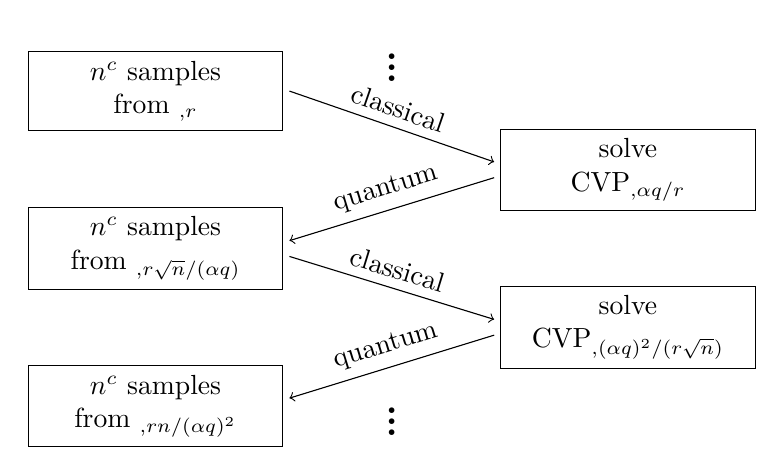
\begin{tikzpicture}
% Define the first block
\node[draw, minimum width=3cm, minimum height=1cm, text width=3cm, align=center] at (-1,0) {$n^c$ samples \\ from $\D_{\Ll, r}$};

% Define the second block
\node[draw, minimum width=3cm, minimum height=1cm, text width=3cm, align=center] at (5,-3) {solve \\ \prob{CVP}$_{\Lld, (\alpha q)^2/(r \sqrt{n})}$};

% Define the third block
\node[draw, minimum width=3cm, minimum height=1cm, text width=3cm, align=center] at (-1,-2) {$n^c$ samples \\ from $\D_{\Ll, r \sqrt{n}/(\alpha q)}$};

% Define the fourth block
\node[draw, minimum width=3cm, minimum height=1cm, text width=3cm, align=center] at (5,-1) {solve \\ \prob{CVP}$_{\Lld, \alpha q/r}$};

% Define the fifth block
\node[draw, minimum width=3cm, minimum height=1cm, text width=3cm, align=center] at (-1,-4) {$n^c$ samples \\ from $\D_{\Ll, r n/(\alpha q)^2}$};

% Draw the lines between the blocks
\draw[->] (0.7, 0) -- node[sloped, above] {classical} (3.3, -0.9);
\draw[->] (3.3, -1.1) -- node[sloped, above] {quantum} (0.7, -1.9);
\draw[->] (0.7, -2.1) -- node[sloped, above] {classical} (3.3, -2.9);
\draw[->] (3.3, -3.1) -- node[sloped, above] {quantum} (0.7, -3.9);

% Add dots
\node[above=0.5cm] at (2, -0.5) {\Huge $\vdots$};
\node[above=0.5cm] at (2, -5) {\Huge $\vdots$};
\end{tikzpicture}
}
\end{figure}

We now present heavily simplified version of the algorithm that, when given a polynomial amount of samples from the discrete Gaussian, gives us a solution to the \prob{CVP} to within error of $\alpha q /(\sqrt{2} r)$ to the dual lattice $\Lld$.
\begin{lemma}[Step 1 - classical]\label{classical}
        Let $\epsilon = \epsilon(n)$ be a negligible function, $\alpha > 0$ real, and $q \geq 2$ be an integer. Assume that we have access to an oracle that solves LWE$_{q, \Psi_{\leq \alpha}}$ given a polynomial number of samples. Then, there exists an efficient algorithm that, given an $n$-dimensional lattice $\Ll$, a number $r > \sqrt{2}q \eta_{\epsilon}(\Ll)$, and a polynomial list of samples from $\text{D}_{\Ll,r}$, solves \prob{CVP}$_{\Ll^{\vee},\alpha q/(\sqrt{2}r)}$.
\end{lemma}
Our goal is, given a point $\bm{x}$ close enough (precisely within $\alpha q/(\sqrt{2}r)$) to $\Lld$, construct an instance of a $A_{\bm{s}, \Psi_{\leq \alpha}}$ where the $\bm{s}$ will depend on $\bm{x}$. After polynomial amount of such samples, we can then use our oracle to recover $\bm{s}$ and consecutively $\bm{x}$. We say an algorithm solves \prob{CVP}$_{\Ll, d}$ if, given any point $\bm{x} \in \R^n$ within distance $d$ of $\Ll$ it gives $\bm{y} \mod q \in \Z_q^n$, the coefficient vector of the closest vector to $\bm{x}$ reduced modulo $q$\footnote{This is technically a solution to \prob{CVP}$^{(q)}_{\Ll, d}$ - regular \prob{CVP} but reduced modulo $q$. However as we will see later in the proof, there exists a reduction from one to another.}.

The following proof is a simplified version of the proof of Lemma 3.11 from \cite{regev} where we skip few technical details. For all of them, the reader is redirected to the original.
\begin{proof}
        We start with a sample vector $\bm{v} \in \Ll$ from D$_{\Ll, r}$ and set $\bm{a} = \Ll^{-1} \bm{v} \mod q$ - its coefficient vector (notice that we are slightly abusing the notation here using $\Ll$ as the matrix representing the lattice). We note at this point that it is in fact enough to find solution modulo $q$ as there exists an algorithm iterating over the coefficients along with (for example) Babai's nearest plane algorithm (see \cite{babai}) to obtain the full, unreduced solution. For the details, see \cite{regev} Lemma 3.5. We now output
        \begin{equation} (\bm{a}, \langle \bm{x}, \bm{v} \rangle + e' \mod q) \end{equation}
        where the $e' \in \R^n$ is chosen from a continuous normal distribution with deviation $\alpha/(\sqrt{2} \pi)$. We claim now that our output is within negligible statistical distance of $A_{\bm{s}, \Psi_{\leq \alpha}}$ for $\bm{s} = (\Lld)^{-1}\bm{y} \mod q$.

        To see this, first note that $\bm{a}$ is a uniform sample (\cite{regev}, Claim 3.8). This is because $r \geq \eta_{\epsilon}(\Ll)$ and by our discussion in \ref{smoothing}, the $\D_{\Ll, r}$ will behave like a uniform distribution. Let us now fix $\bm{a}$ and consider $\bm{y} = \bm{x} - \bm{e}$. Then
        \[ \langle \bm{x}, \bm{v} \rangle + e' \mod q = \langle \bm{e}, \bm{v} \rangle + \langle \bm{y}, \bm{v} \rangle + e' \mod q. \]
Focusing now on the second term, we observe that
\[ \langle \bm{y}, \bm{v} \rangle = (\Lld)^{-1} \langle \bm{y}, \bm{v} \rangle \Lld =  \langle (\Lld)^{-1}\bm{y}, \Ll^{-1} \bm{v} \rangle = \langle \bm{s}, \bm{a} \rangle \]
since $\Ll^{-1} = (\Lld)^T$.

To finish the proof we need to show that the remaining term $\langle \bm{e}, \bm{v} \rangle + e'$ is distributed within negligible statistical distance of $\Psi_{\leq \alpha}$. This is obtained by noting that summing two normal distributions with the standard deviation less than the smoothing parameter, gives us a distribution that is indeed close enough to $\Psi_{\beta}$ for some $\beta \leq \alpha$ as desired. This is Claim 3.10 in the original paper by Regev.
\end{proof}
\begin{proposition}[Step 2 - quantum]\label{quantum}
        There exists an efficient quantum algorithm that, given any $n$-dimensional lattice $\Ll$, a number $d < \lambda_n (\Lld)/2$, and an oracle that solves \prob{CVP}$_{\Lld,d}$, outputs a sample from D$_{\Ll,\sqrt{n}/(\sqrt{2}d)}$.
\end{proposition}

Lastly, we can finish the proof of Theorem \ref{main} by presenting the following proposition that provides reduction from \prob{SIVP} and \prob{GapSVP} to \prob{DGS}.

\begin{proposition}
        Let $\Ll$ be an $n$-dimensional lattice and let $r$ be such that $r \geq \sqrt{2}\eta_{\epsilon}(\Ll)$ where $\epsilon \leq \frac{1}{10}$. Then, the probability that a set of $n^2$ vectors chosen independently from D$_{\Ll,r}$ contains no $n$ linearly independent vectors is exponentially small.
\end{proposition}

\subsubsection{Pseudorandomness of LWE}
In this section we will prove that the search version of LWE - Definition \ref{slwe} - to the decision version - Definition \ref{dlwe}. More precisely, if our sample is of the form $(\bm{a}, b)$, there is no way for us to tell if $b$ is uniform or actually $b = \langle \bm{a}, \bm{s} \rangle + e$ for some secret $\bm{s}$ and small error $e$.

In general, the decision version is considered more suitable for cryptographic purposes because it is often easier to analyze and prove security guarantees for. For many cryptographic problems, it is computationally infeasible to find the solution to the search version, but it is possible to determine the correct answer to the decision version with high probability. Thus, cryptographic schemes are often designed based on decision versions of hard computational problems.

The statement can be phrased as follows.
\begin{theorem}[\cite{regev}, 4.2 - Decision to Search]\label{s-to-d}
        Let $n \geq 1$ be some integer, $2 \leq q\leq \alg{poly}(n)$ be a prime, and $\chi$ be some distribution on $\Z_q$. Assume that we have access to procedure \prob{W} that for all $\bm{s}$ accepts with probability exponentially close to 1 on inputs from $A_{\bm{s},\chi}$ and rejects with probability exponentially close to 1 on inputs from U. Then, there exists an efficient algorithm \prob{W'} that, given samples from $A_{\bm{s},\chi}$ for some $s$, outputs $\bm{s}$ with probability exponentially close to 1.
\end{theorem}

In other words, if we have an oracle (called procedure in this theorem) that solves the decision-LWE, then there is an efficient (running in polynomial time) algorithm that outputs us the secret $\bm{s}$ used for the generation of the sample (if the sample was indeed taken from $A_{\bm{s}, \chi}$).

\begin{proof}
        We are given a sample $(\bm{a}, b)$ and an oracle that tells us whether this element was chosen uniformly at random, or whether $b$ is related to $\bm{a}$ via $b = \langle \bm{a}, \bm{s} \rangle + e$. Note that by definition in both cases $\bm{a}$ is chosen uniformly from $\Z_q^n$. The idea to obtain the secret $\bm{s}$ is relatively simple. We pick some element $k \in \Z_q^n$ and check coordinate by coordinate if this is the respective coordinate of our key $\bm{s}$. The procedure is identical for each coordinate hence we will only consider the case of the first one. Pick any $k$ as before and consider the transformation $(\bm{a} + (l, 0, \cdots, 0), b +k \cdot l)$ for $l\in Z_q^n$ chosen uniformly at random. We have now three cases to consider.
        \begin{enumerate}
                \item Our original sample was in fact taken from uniform distribution. Then it is easy to see that the transformation maps it again to uniform and nothing is changed. In this case, there is no $\bm{s}$ to be found and we terminate.
                \item The sample was taken from the $A_{\bm{s}, \chi}$ distribution. Then either:
                        \begin{enumerate}
                                \item $k = s_1$. In this case, the sample is mapped back to $A_{\bm{s}, \chi}$ because \[ \langle (a_1 + l, a_2, \cdots, a_n), \bm{s} \rangle + e = \langle \bm{a}, \bm{s} \rangle + l \cdot s_1 + e = b + k \cdot l.\] We can now proceed with $s_2$ in a similar manner.
                                \item Or $k \neq s_1$ in which case the sample is mapped to a uniform distribution and oracle tells us we picked wrong. Note that this requires our $q$ to be prime because otherwise it might happen that $a_1 \cdot k = a_1 \cdot s_1$ as either of the three could be a zero divisor. We have therefore picked wrong $k$ and we need to pick another one.
                        \end{enumerate}
        \end{enumerate}
        Note that by the choice of our $q \leq \alg{poly}(n)$, we can try all of them.
\end{proof}

%There are two other results that, when combined with the previous lemma, give us hardness of decision LWE based on \textit{worst-case} lattice problems like \prob{SIVP} and the \prob{GapSVP}. These results are:
%\begin{enumerate}
%       \item \textit{Continuous} $\iff$ \textit{Discrete}. We used distributions that are discrete over the integers modulo some integer. However it does not matter if we were to pick a continuous one and never discretize it.
%       \item \textit{Average-case} $\iff$ \textit{Worst-case}. All the results proved in previous section didn't assume anything about problems and the running time of the algorithms used for solving them. As proved in Lemma 4.1 in \cite{regev}, the LWE problem is as hard as solving those problems in the worst-case.
        %\item \textit{LWE} and \textit{DGS} $\iff$ Hard lattice problems like \textit{SIVP} and the decision version of shortest vector problem \textit{GapSVP}.
%\end{enumerate}

%All those results combined, give us the following lemma

\subsubsection{LWE cryptosystem}
Now that we have a solid hardness assumptions, we can attempt to construct a cryptosystem that employs those results. The following public key cryptosystem was presented in the same paper. To keep the notation consistent with previous section, we will slightly deviate from the original.

We begin by specifying our parameters. Let us denote by $n$ our security parameter. As before, the scheme is characterized by two integers $m$ and $q$ and a probability distribution $\chi$ over $\Z_q$. To now make the scheme secure and correct, we should choose $q$ prime between $n^2$ and $2n^2$, $m = (1 + \epsilon)(n + 1) \log q$ for some arbitrary constant $\epsilon > 0$. We define the distribution $\chi$ to be $\bar{\Psi}_{\alpha (n)}$ (the discretized Gaussian distribution $\Psi_{\alpha}$) where $\alpha (n) = o(1/(\sqrt{n} \log n))$ (recall from Section \ref{hardness} that it means $\lim_{n\to\infty} \alpha (n) \cdot \sqrt{n} \log n = 0$). The scheme is presented in Table \ref{lwe-enc}.

\begin{table}[ht]
        \centering
\begin{mdframed}
$\alg{KeyGen:}$
\begin{itemize}
    \item Choose $\bm{s} \in \Z^n_q$ uniformly at random. This is the \textbf{private key}.
    \item For $i = 1, \dots, m$ choose $m$ vectors $\bm{a}_i \in \Z^n_q$ independent from the uniform distribution. Additionally choose $m$ elements $e_i \in \Z_q$ independently according to $\chi$. The \textbf{public key} is the array of $m$ vectors of the form $(\bm{a}_i, b_i)$ where each $b_i$ is given by $b_i = \langle \bm{a}_i, \bm{s} \rangle + e_i$.
\end{itemize}
$\alg{Encrypt:}$\\
To encrypt a single bit we choose a random set $S$ uniformly among all $2^m$ subsets of $\{1, \dots, m\}$. The encryption is $(\sum_{i \in S} \bm{a}_i, \sum_{i \in S} b_i)$ if the bit is 0, and $(\sum_{i \in S} \bm{a}_i, \lfloor q/2 \rfloor + \sum_{i \in S} b_i)$ otherwise. \\
$\alg{Decrypt:}$\\
The decryption of a pair $(\bm{a}, b)$ is 0 if $b - \langle \bm{a}, \bm{s} \rangle$ is closer to 0 than to $\lfloor q/2 \rfloor$ modulo~$q$.
\end{mdframed}
\caption{LWE encryption scheme}
\label{lwe-enc}
\end{table}

\begin{example}
    Almost exactly like in the Example \ref{lwe_ex}, set $n = 4$, $q=17$ and $m=4$. We pick our \textbf{secret key} $\bm{s} = (2,1,3,7)$ and artificially (i.e. by design and not uniformly at random) pick
    \[ \bm{A} = [\bm{a}_1 \, \bm{a}_2 \, \bm{a}_3 \, \bm{a}_4] = 
        \begin{pmatrix}1 & 16 & 4 & 5\\
                        16 & 4 & 5 & 1 \\
                        4 & 5 & 1 & 16 \\
                        5 & 1 & 16 & 4
        \end{pmatrix}. \]
        Take $e_1 = e_2 = 1$ and $e_3 = e_4 = -1$. Now we can compute the \textbf{public key} 
        \[ \bar{\bm{A}} = \begin{bmatrix} \bm{A} \\ \bm{b} \end{bmatrix} = 
        \begin{bmatrix} \bm{A} \\ \langle \bm{a}_i, \bm{s} \rangle + e_i \end{bmatrix}  = 
        \begin{pmatrix} 1 & 16 & 4 & 5 \\
            16 & 4 & 5 & 1 \\
            4 & 5 & 1 & 16 \\
            5 & 1 & 16 & 4 \\
            15 & 8 & 8 & 11
        \end{pmatrix}.
        \]
    To now encrypt a bit 1, we can take as our $S$ the set $\{1,2,4\}$ and output the encryption as
     \[(\bm{a}, b)^T = \begin{pmatrix} 1 + 16 + 5\\ 
                16 + 4 + 1\\
                4 + 5 + 16 \\
                5 + 1 + 4 \\
                \lfloor 17/2 \rfloor + 15 + 8 + 11 \\
                \end{pmatrix} = \begin{pmatrix} 5 \\ 4 \\ 8 \\ 10 \\ 0  \end{pmatrix}.
            \]

            Decryption is just another simple computation, we first compute $\langle \bm{a}, \bm{s} \rangle = 108 \equiv 6 \mod 17$ which gives us $b - \langle \bm{a}, \bm{s} \rangle = 0 - 6 \equiv 11 \mod 17$. Let us compare the distances to 0 and $\lfloor q/2 \rfloor = 8$. $|11 - 17| = 6 > 3 = |11 - 8|$. Hence, our decryption worked correctly as indeed, the result is closer to $\lfloor q/2 \rfloor$ than to 0. Finally, we output 1 as the decryption of our message and we are done.
\end{example}

\paragraph{Analysis}
Now, that we have finally defined a cryptographic scheme we need to verify it. The two remaining questions we now have are first, is this scheme correct? That is, does the decryption algorithm correctly evaluate back to the original message? This is much more difficult to prove compared to the scheme over the integers presented in \ref{int_she}. The following is a somewhat simpler version of Claim 5.2 in \cite{regev}.
\begin{lemma}[Correctness]
        For the above choice of parameters and $e$ following the $\bar{\Psi}_{\alpha}$ distribution we have
        \begin{equation} \Pr_{e \sim \bar{\Psi}_{\alpha}} \Big[ |e| < \Bigl \lfloor \frac{q}{2} \Bigr \rfloor /2 \Big] > 1 - \delta(n) \end{equation}
    for some negligible function $\delta(n)$.
\end{lemma}
\begin{proof}
        Note that if not for the error term, the decryption would always be correct. Hence we need to pay attention to the case where the error term is greater than $q/4$. Since there are $m$ such terms, each with standard deviation of $\sigma^2 = \alpha q$, we can use Proposition \ref{gauss_sum} to show that if $X_i \sim \mathcal{N}(0, \alpha q)$ are i.i.d. for $i \in [m]$, then the sum
        \[ \sum_{i \in [m]} X_i \sim \mathcal{N}(0, \sum_{i \in [m]} \sigma^2) = \mathcal{N}(0, m \cdot \sigma^2)\]
        is distributed with standard deviation equal to $\sqrt{m} \alpha q < q / \log(n)$ and the probability that such sample is greater than $q/4$ is negligible.
\end{proof}
An example of a normal distribution with standard deviation $\sigma^2 = q/\log n$ and mean 0 can be seen in Figure \ref{1d-gaussians}. The shaded region corresponds to $|e| > q/4$. At the begining, for $n$ not as big, we can notice that the area does not necessarily correspond to an intuitive notion of ``negligible''. However, the definition concerns the asymptotic behavior of $n$ and indeed, we can see the area becomes quite small. One might even call it ``negligible''.% The Python script used to generate these figures can be found in Appendix \ref{appendix:code}.

\begin{figure}
        \caption{1 dimensional Gaussian with standard deviation $\sigma^2 = q/\log n$ for:}
        \label{1d-gaussians}
        \centering
        \begin{subfigure}{.5\textwidth} 
                \centering
                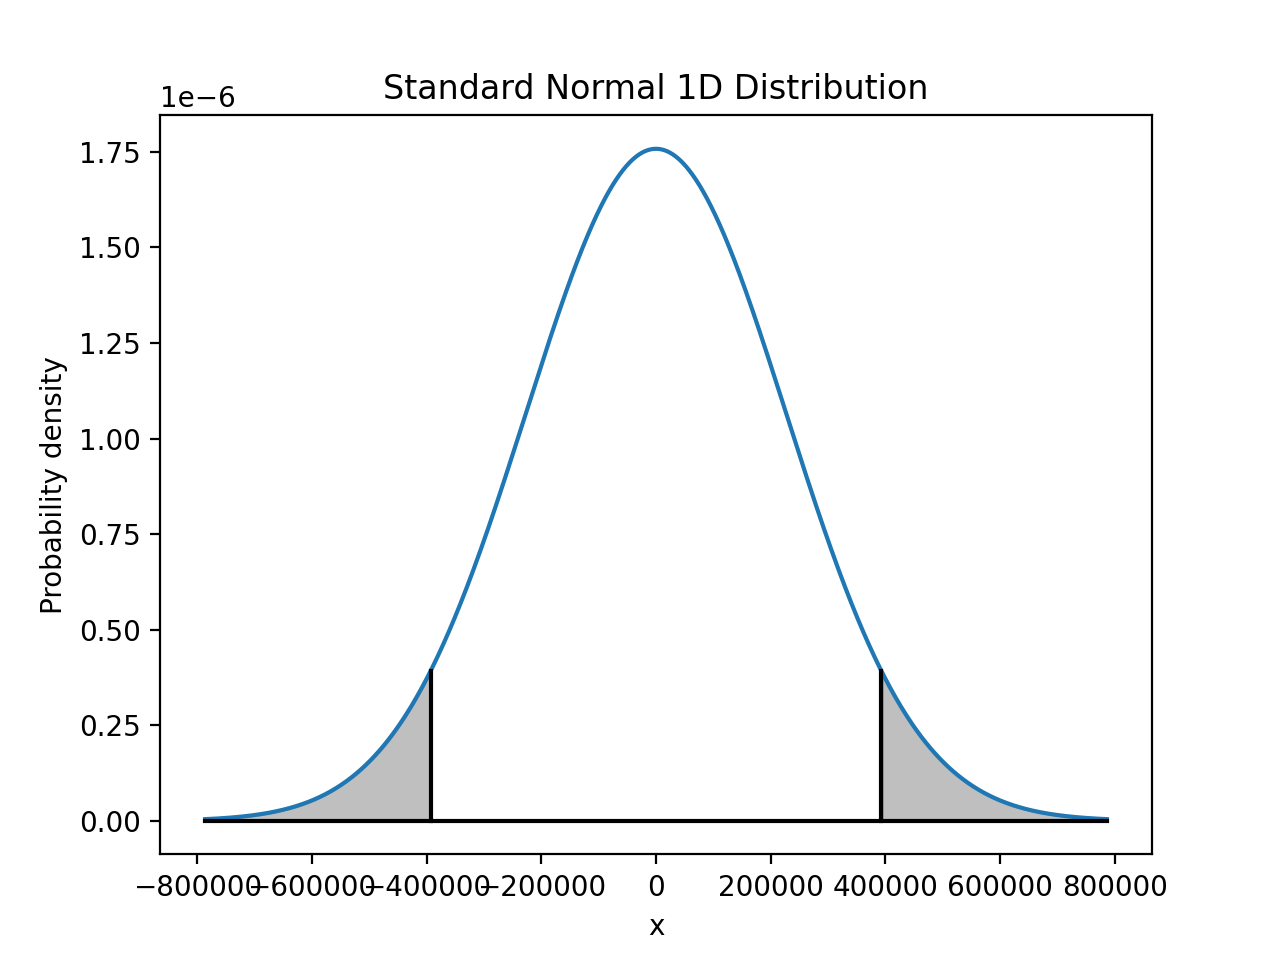
\includegraphics[scale=0.5]{gaussian1d-1024.png}
                \caption{$n = 1024$}
        \end{subfigure}%
        \begin{subfigure}{.5\textwidth}
                \centering
                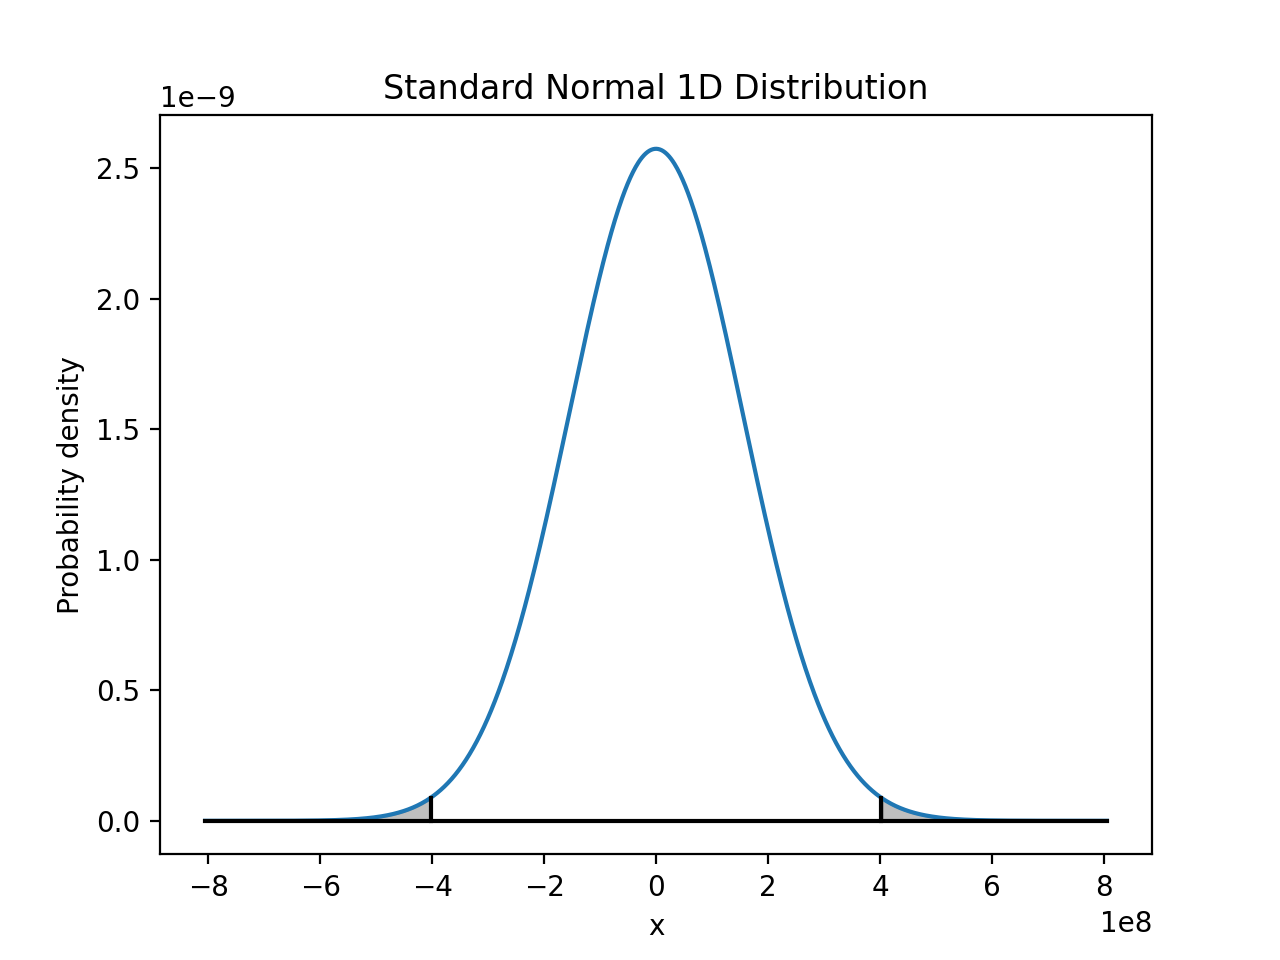
\includegraphics[scale=0.5]{gaussian1d-32768.png}
                \caption{$n = 32768$}
        \end{subfigure}
\end{figure}

This, in turn, implies that (this is Lemma 5.1)
\begin{lemma}
    The decryption is correct with probability $1 - \delta(n)$ where the $\delta(n)$ is some negligible function.
\end{lemma}

\begin{proof}
    Consider first the encryption of 0. It is given by $(\bm{a}, b)$ with $\bm{a} = \sum_{i \in S}\bm{a}_i$ and $b = \sum_{i \in S} b_i = \sum_{i \in S} \langle \bm{a}_i, \bm{s} \rangle + e_i$. Then the decryption gives us precisely $b - \langle \bm{a}, \bm{s} \rangle = \sum_{i \in S} e_i$. By our assumption, $\big| \sum_{i \in S} e_i \big| < \bigl \lfloor \frac{q}{2} \bigr \rfloor /2$ with probability at least $1 - \delta(n)$. In that case, it is closer to 0 than $\bigl \lfloor \frac{q}{2} \bigr \rfloor$ and thus correctly decrypts to 0. The case for the encryption of 1 is similar.
\end{proof}

Note that it seems almost trivial that we decrypt correctly, the scheme was designed in that way. This is only the case when we know the secret key $\bm{s}$ that is definitely not know to the public. This ties closely to the second and last question, that is, how secure the scheme is? We have established hardness based on average and worst-case lattice problems. However, it might be the case that our choice of parameters required for correctness, hinders on the security. This is resolved with the following theorem. Let us first define some required terminology.

\begin{proposition}[\cite{regev}, Lemma 5.4]
    For any $\epsilon > 0$ and $m \geq (1 + \epsilon)(n + 1) \log q$, if there exists a polynomial time algorithm $\alg{W}$ that distinguishes between encryptions of 0 and 1 then there exists a distinguisher $\alg{Z}$ that distinguishes between $A_{\bm{s}, \chi}$ and $U$ for a non-negligible fraction of all possible $\bm{s}$.
\end{proposition}
Note that this closely relates to the last lemma from the previous section on the hardness of LWE. For a thorough and less technical analysis than the one given in the original paper, the reader is encouraged to look into section 5.4 in \cite{Micci2009}.

\subsubsection*{Epilogue}
\krzys{do last if theres time}
Until the day of writing this paper, LWE is one of the most influential schemes that can be used for post-quantum cryptographic schemes. It was used as a basis for schemes like the one introduced in \cite{ot-lwe} (along with an oblivious transfer protocol), \cite{lwe-scheme1} or \cite{lwe-scheme2}. However, arguably the most important contribution, was that of laying groundwork for the \textit{ring}-LWE scheme introduced in the next section. We will now present few alternatives to the results and proofs presented here.\\

\iffalse
Let us begin with the proof of the main theorem, namely, the quantum part. At some point, we would like to find entirely \textit{classical} and efficient reduction algorithm that proves the hardness of the problem. This is because we understand classical computation in much more detail than its quantum equivalent. Using classical computers we have cracked Enigma and landed on the moon. In the meantime, only recently a factorization of the integer 15 was achieved on a quantum computer using Shor's algorithm - see \krzys{find source of that statement}. Returning to the reduction problem, Chris Peikert in his paper \cite{peikert_classical} from 2009 has done exactly this. However, it was done in a somewhat ``inefficient'' way. That is, exponentially many samples are needed in the classical reduction compared to polynomial amount in the quantum version. For more details see the paper by Peikert and compare it with the original approach from Regev. It remains an important open question \krzys{also not sure about that} till this day, if the reduction can be made efficiently fully classical.
\fi
